\section{Object Versioning} \label{chapter:APPROACH}

% This chapter introduces our approach to preserving access to previous states in systems like the Lively Kernel.
% Our approach to object versioning is based on immutable object copies and version-aware references that manage versions of objects transparently.\\
% This chapter introduces our approach, as well as a design to implement version-aware references with proxies.
% \subsection{Object Versions} \label{sec:APPROACH:1}

A previous version of an object is, in the simplest case, a copy of the object before its state was manipulated.
Consider an object representing an address with fields for \lstinline{street}, \lstinline{number}, and\lstinline{city}.
As the user interacts with the object, its state changes and different \emph{versions} (i.e., co-existing copies) of the object are created (\autoref{fig:VersionPreserved}.)
The two objects have no additional information to indicate to which version of the system they belong, nor do they store any information showing that one is a copy of the other.

\begin{figure}[h]
    \centering
    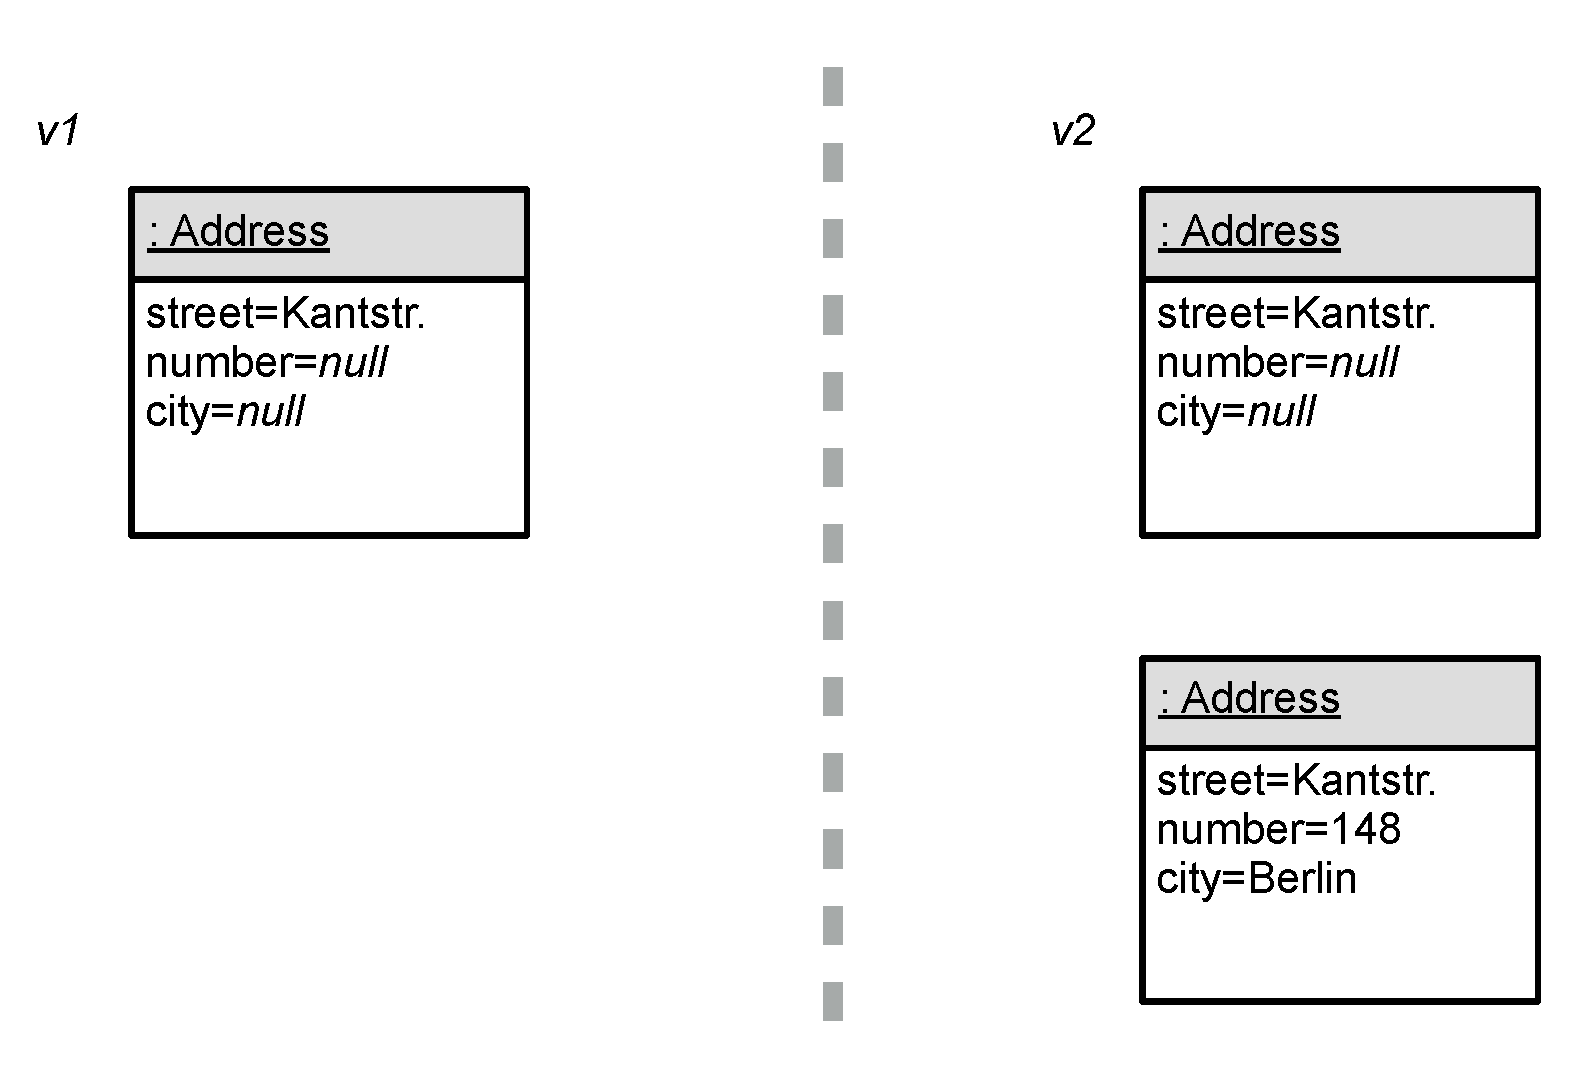
\includegraphics[width=0.7\columnwidth]{figures/4_approach/3_previousVersionPreserved.pdf}
    \caption{Preserving the previous version of the \lstinline{address} object.}
    \label{fig:VersionPreserved}
\end{figure}


To be able to access different versions of an object, its previous states need to be kept alive through our \emph{version-aware references}.
Version-aware references behave like ordinary references, but they know which versions of an object are available and always resolve to one of those based on context information.
When, for example, an object representing a person references its \lstinline{address}, we use a version-aware reference to resolve to either \emph{v1} or \emph{v2} of the address, as shown in \autoref{fig:VersionAwareReferenceFollowingVersion2}.

\begin{figure}[h]
    \centering
    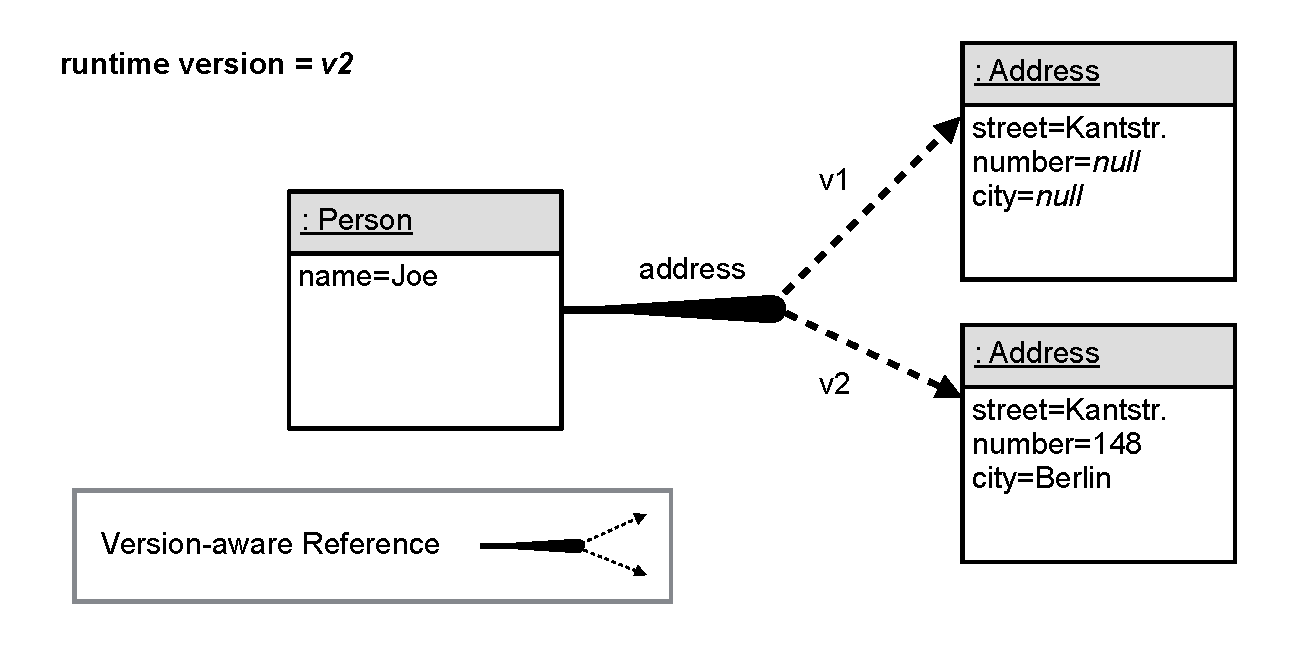
\includegraphics[width=0.8\columnwidth]{figures/4_approach/5_versionAwareReferenceFollowingVersion2.pdf}
    \caption{A version-aware reference relates a \lstinline{person} object to two versions of its \lstinline{address} property.}
    \label{fig:VersionAwareReferenceFollowingVersion2}
\end{figure}

In the same way, multiple version-aware references can be resolved as one path through a graph of versions.
Through different possible traversals of the version-aware object graph, different versions of the system emerge.
The version-aware references all choose versions of objects that belong to the same system state.
\autoref{fig:ObjectGraphWithReferencesResolvedAlongVersion2} shows such an object graph.

\begin{figure}[h]
    \centering
    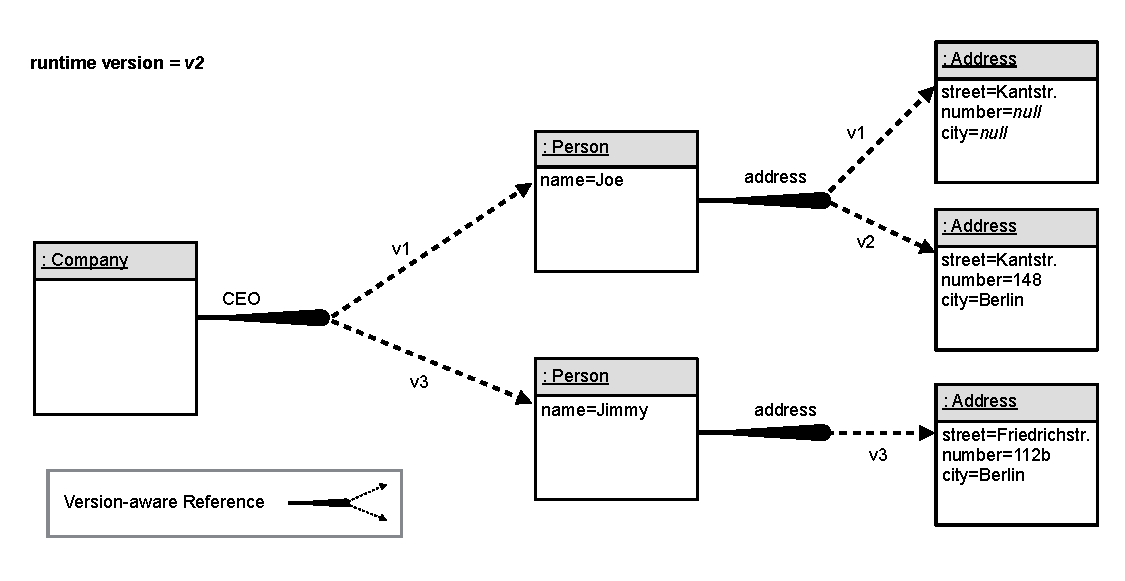
\includegraphics[width=\columnwidth]{figures/4_approach/6_objectGraphWithVersonAwareReferences.pdf}
    \caption{An object graph with version-aware references.}
    \label{fig:ObjectGraphWithReferencesResolvedAlongVersion2}
\end{figure}


\subsection{Versions of the System}
\label{sec:versions-system}

To establish system versions from version-aware object graphs, the version-aware references resolve to different object versions dynamically based on a \emph{version identifier}.
As this identifier changes, the version-aware references resolve to other versions of objects.
In order to undo a change made in version \emph{v2} of the system, the version identifier is simply set back to \emph{v1}.

Given the example situation from \autoref{fig:ObjectGraphWithReferencesResolvedAlongVersion2}, the following statement would refer to three different values depending on the version identifier:

\begin{code}
Company.CEO.address.number
\end{code}

Evaluating the statement in version \emph{v1} would return the value \lstinline{null}, in version \emph{v2} the value \lstinline{148}, and in version \emph{v3} the value \lstinline{112b}.
Note that no \emph{v2} reference exists from \lstinline{Company} to a \lstinline{ceo}.
Version identifiers have a \emph{predecessor} and a \emph{successor}, so when no current version is available, the most recent available version can be found.
This optimization allows to only create new versions of objects when necessary.

The version identifier needs to be accessible to the version-aware references.
It might be a global (to have a single active version of the system), but could also be thread-local, or in the dynamic scope of an execution.
However, it must not be changed while a versioned object graph is traversed.
This is automatically true only for dynamically scoped version identifiers.

To enable our approach to actually re-establish a particular version of the system with our approach, all mutable objects must only be accessed via version-aware references. To satisfy this requirement, we propose a system transformation that uses proxy objects as references.

\subsection{Ubiquitous Proxies as Version-aware References} \label{sec:APPROACH:2}

Applications written in JavaScript typically have to work on a variety of client \acp{vm} included in different Web browsers.
This makes a language-level implementation preferable to an implementation of \emph{alternative references} in each JavaScript \ac{vm}\@.
We use proxies pointed to by \emph{ordinary references} to delegate to object versions transparently, as shown in \autoref{fig:ProxyBasedVersionAwareReference}.
Each property accessed on a proxy is forwarded transparently to the correct version of the object.
Thus, proxies in this design are \emph{virtual objects}~\cite{VanCutsem2010PDP}; they do not stand in for a specific object, but can forward intercepted interactions to any object.

\begin{figure}[h]
    \centering
    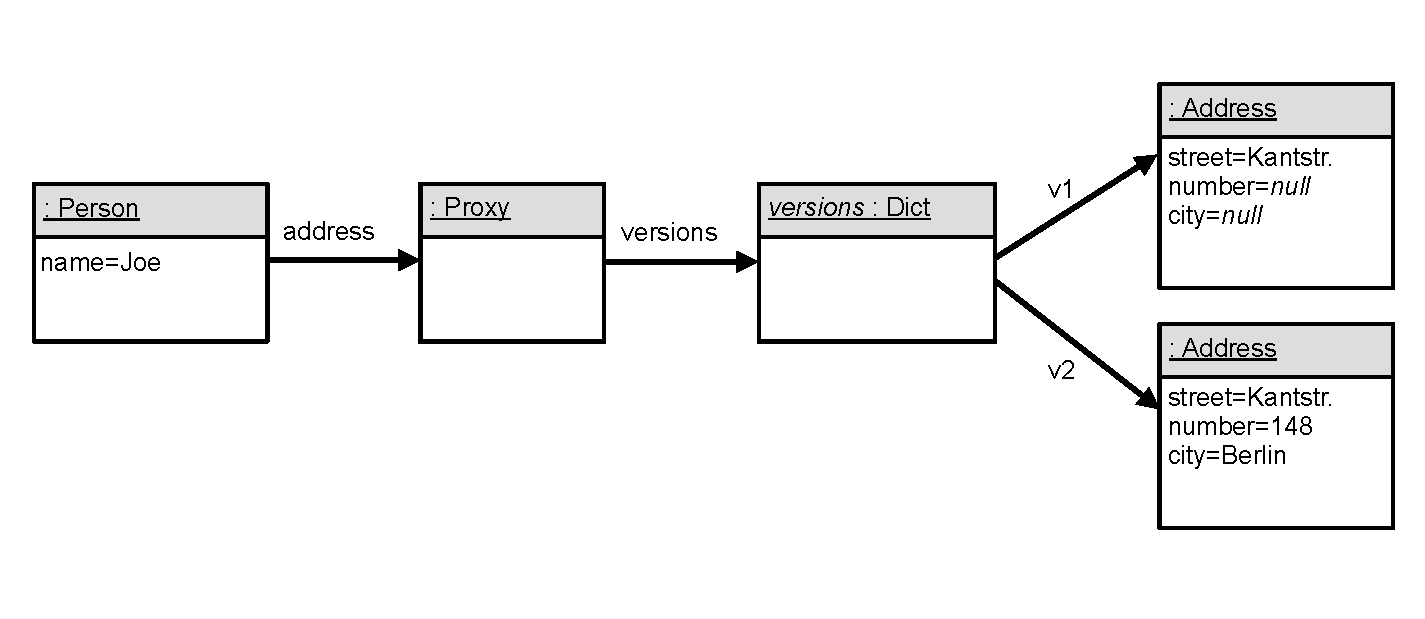
\includegraphics[width=\columnwidth]{figures/4_approach/7_proxyBasedVersionAwareReference.pdf}
    \caption{Using a proxy as version-aware reference to connect a \lstinline{person} object to two versions of an \lstinline{address} object.}
    \label{fig:ProxyBasedVersionAwareReference}
\end{figure}

The proxies fulfill three responsibilities:
\begin{enumerate}
    \item They know which versions are available for a particular object.
    \item They choose a particular version among all available dynamically using context information.
    \item They forward all interactions transparently to a chosen version.
\end{enumerate}

As mentioned in \autoref{sec:versions-system}, we use a source transformation to interpose proxies consistently between all mutable objects.
Our transformation wraps object literals and constructor functions into proxies, so all expressions that create new objects transparently return proxies.
The reference to the initial version of an object is only available to the proxy; the reference to the proxy is passed around instead.
Consequently, all references that would usually point to the same object point to the same proxy.
This way, proxies provide object identity.
Checks that would usually compare an object to another objects now compare a proxy to another proxy.

Although keeping many versions around might put more pressure on the garbage collector, no special care has to be taken to release versions that are no longer required.
All object versions are referenced through a single proxy, so the versions get garbage collected with the proxy when it is no longer reachable.
So if you consider the \lstinline{Company} from \ref{fig:ObjectGraphWithReferencesResolvedAlongVersion2}, once you delete \emph{v1} of the \lstinline{ceo} reference, both \emph{v1} and \emph{v2} of the address object are collected.

The current version identifier of the system is accessible to the proxies.
The proxies forward to the same version of the object as long as the identifier remains constant.

\emph{To re-establish the previous version}, the version identifier is set to its predecessor.

\emph{To preserve the current version}, the version identifier is set to a new version.
The proxies forward interactions to other object versions or, when no such version of the object exist, create new versions.
Note that new versions are only necessary when a proxy is about to delegate manipulations.
As long as the state of an object is only read, the proxy reports values from a previous version as the old version of the object still reflects the current state.
To create a new version, a proxy copies the most recent previous version of the object.

Such a situation is shown in \autoref{fig:NewVersion}.
In a new version \emph{v3} of the system the proxy intercepts a manipulation, but has no object version it can forward to.
It therefore copies the most recent version of the object and forwards to the copy.

\begin{figure}[h]
    \centering
    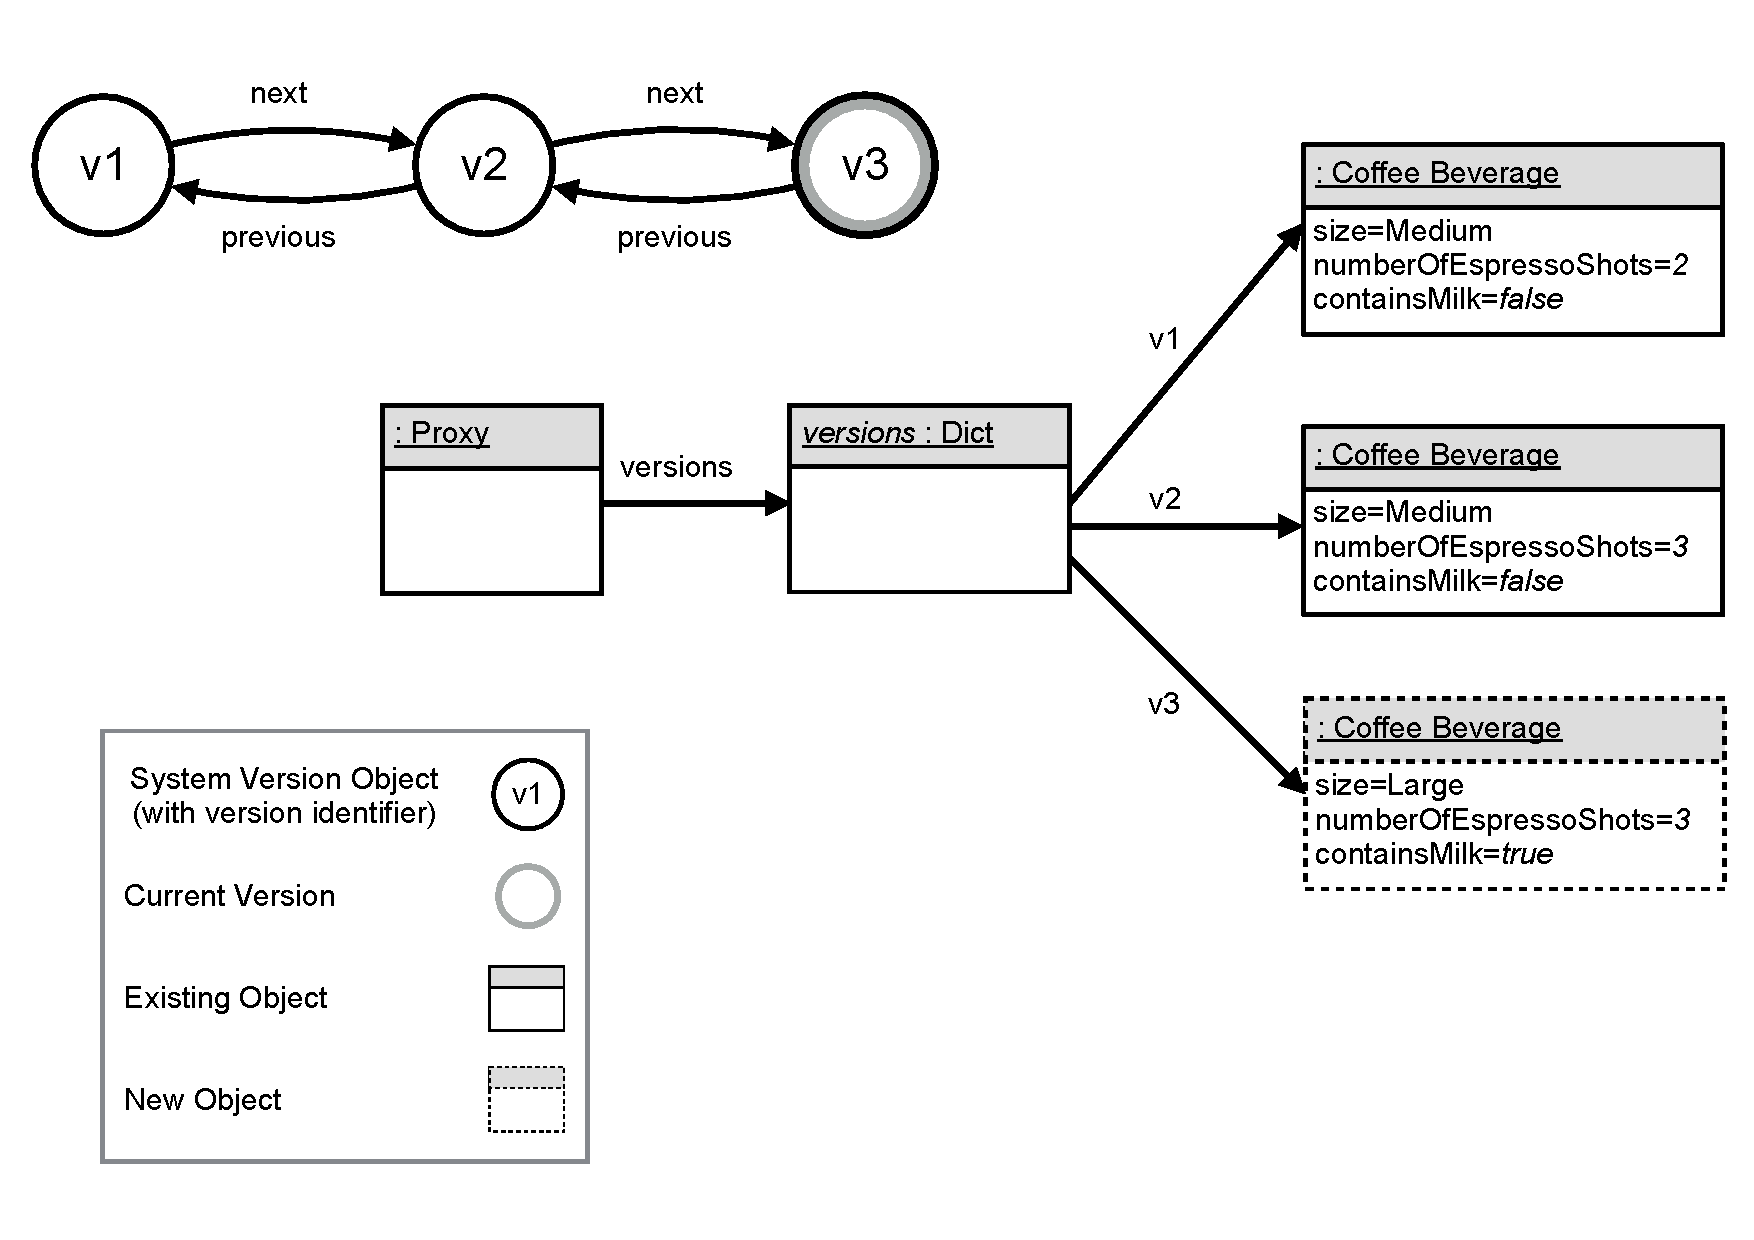
\includegraphics[width=0.86\columnwidth]{figures/4_approach/10_newVersionOfAnObject.pdf}
    \caption{A new version of an object is created for a new version of the system.}
    \label{fig:NewVersion}
\end{figure}


\paragraph{Limitations}

The current design allows to preserve and re-establish versions of the system.
Without further components, however, these versions only exist in memory and are not stored to disk.

Our current design does not support multiple predecessors or successors.

Another limitation of the current design is that the state of previous versions can be changed.
New versions of objects are not affected by changes to previous versions, but changes to object versions that have not been copied shine through in subsequent versions of the system.

In the future, the versioning might allow for branches and merging.
Changes to previous states could then be handled in branches that programmers may or may not merge into future versions.

%%% Local Variables:
%%% mode: latex
%%% TeX-master: "../main"
%%% End:
